\chapter{Subsystem Implementation\label{cha:implementation}}

The purpose of this chapter is to document the work completed in the implementation phase of the project. Implementation was carried out with three major goals in mind:

\begin{enumerate}
  \item To verify the system design, and compare the results with those desired in Ch. \ref{cha:goals};
  \item To use the results as working prototypes for the demonstration and communication of various aspects of the project; and
  \item To produce a first iteration of usable modules to be integrated into the vehicle for competition in May of 2010.
\end{enumerate}

This chapter is broken down into eight sections. First, the simulation and physical implementation of the electro-pneumatic subsystem is discussed. Next, commonalities in the hardware and software implementations are introduced. Then, the hardware and software implementations of the four modules are explained. Finally, the \emph{CAN Diagnostic Tool} is introduced. This tool was implemented to allow for in-place testing of the four modules, and is complex enough to warrant inclusion in the implementation.

\section{Electro-Pneumatic System\label{sec:electropneumatic_implementation}}

\nomenclature{PID}{Proportional-Integral-Differential}

Several steps were taken in the implementation phase to develop a better understanding of the electro-pneumatic's behaviour, and to provide data and models that could be used in the implementation of the controller software. A Simulink model was developed to verify that our fundamental design would work, and to gain further insight into the operation of the electro-pneumatic system. A simple \emph{Proportional-Integral-Derivative} (PID) controller block was used to show that the closed-loop system was inherently stable.

\subsection{Simulation with Simulink}

An overview of the Simulink model used to simulate the electro-pneumatics system is shown in \ref{fig:pneumatics_top_level}. A PID controller block is used in a closed-loop configuration, and the response to a fixed step input is displayed on the scope block. 

\begin{figure}[H]
\centering
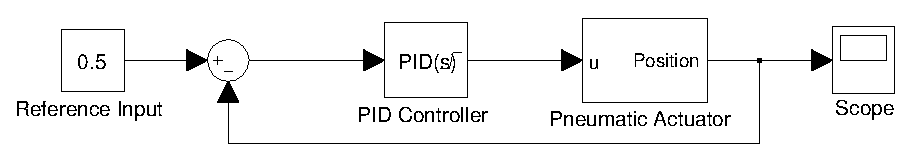
\includegraphics[scale=1]{implementation/figures/pneumatic_modelling1.eps}
\caption{Simulink model of the electro-pneumatic system.}
\label{fig:pneumatics_top_level}
\end{figure}

The three major components of the electro-pneumatic system are the \emph{PWM generator}, the \emph{solenoid valves}, and the \emph{pneumatic actuator}. Models of these systems are described further in the following sections.

\subsubsection{PWM Generator Model}

The PWM generator is used to provide the electrical control signals required by the solenoid valves to open and close. Our model of the PWM generator uses the instantaneous model presented by \citet{valve_models}. This model compares a generated saw-tooth signal $V_{saw}$ with the input signal $V_{in}$ over a time period $T_{saw}$ to obtain the pulse-width-modulated signal $U(t)$. The relationship is illustrated in Eq. \ref{eq:pwm_generation}.

\begin{equation}
\label{eq:pwm_generation}
U\left(t\right) = 
\begin{cases}
1 & V_{in}\left(t\right) \geq V_{saw}\left(t\right) \\
0 & V_{in}\left(t\right) < \left(t\right)
\end{cases}
\end{equation}

The Simulink model which implements Eq. \ref{eq:pwm_generation} can be seen in Fig. \ref{fig:pneumatics_pwm}. The input to the subsystem, shown as \emph{In1}, is $V_{in}$, and the output, shown as \emph{Out1} is the pulse width modulated signal $U(t)$. 

\begin{figure}[H]
\centering
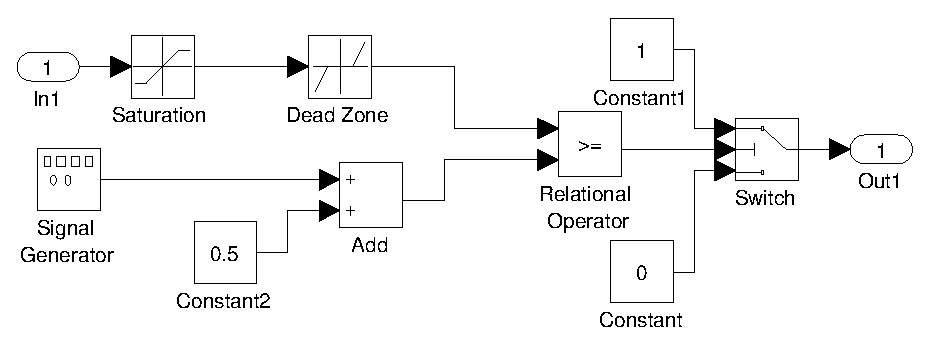
\includegraphics[scale=0.65]{implementation/figures/pneumatic_modelling2.eps}
\caption{Simulink model of the PWM generator.}
\label{fig:pneumatics_pwm}
\end{figure}

A saturation block limits the input signal $V_{in}$ to the range of \unit{[0..1]}{\volt}. A dead-zone block is present to account for the dead-zone present in the solenoid valve response to a PWM signal. If the pulse width is too short, the current through the solenoid cannot generate enough force to open the poppet, so the valve stays shut. This is a parameter of the solenoid valve, and was quantified experimentally by \cite{valve_models} as the minimum input signal $V_{in}$ required to open the valve. \Citet{accurate_position} also account for a minimum possible duty cycle in the solenoid valve input signal, known as $d_{min}$. This value can be calculated as:

\begin{equation}
  \label{eq:pwm_duty_min}
  d_{min}=\left(T_{vr}/T_{PWM}\right)\cdot100\%
\end{equation}

In this case, $T_{vr}$ is the time required by a solenoid valve to respond to an input, and $T_{PWM}$ the period of the PWM signal.

\nomenclature{$d_{min}$}{The minimum possible duty cycle of a solenoid's drive signal that will cause the valve to open.}
\nomenclature{$T_{vr}$}{The time required by a solenoid valve to respond to an input.}

The signal generator block in Fig. \ref{fig:pneumatics_pwm} outputs a triangle wave with peak-to-peak amplitude of \unit{1}{\volt}, which is then offset by \unit{0.5}{\volt}. The relational operator block then compares this with the input signal, and outputs the resulting PWM signal.

\subsubsection{Solenoid Valve Model}

An initial Simulink model of a solenoid valve was constructed based on the modelling equations described by \citet{valve_models} and the standard orifice equations for laminar and choked flow described in \cite{fluid_power}. However, it was too difficult to identify the system parameters cited in \cite{fluid_power} for our specific solenoid valves. The solenoid's data-sheet was not detailed enough, and the straight-forward approach to system identification used by \cite{valve_models} required specialized measuring equipment (such as an instantaneous mass flow meter) that we did not have access to.

The custom Simulink solenoid valve block was replaced with an approximate Simulink ``Simscape'' pneumatic valve block. This block could be configured with data obtained from the valve's data-sheets. 

\subsubsection{Pneumatic Actuator Model}

Simulink's pneumatic actuator subsystem is illustrated in Fig. \ref{fig:pneumatics_actuator}. Pre-built Simulink blocks from the Simscape package were used to model the dynamics of the actuator. \emph{Physical Port 1} (denoted by the octagonal port symbol with a ``1'' inside) in \ref{fig:pneumatics_actuator} represents the air inlet. \emph{Physical Ports 2 and 3} (denoted by the octagonal port symbols with a ``2'' and ``3'' inside, respectively) represent the displacement ports of the cylinder. \emph{Regular Port 1} (denoted by the rounded port symbol with a ``1'' inside) is used to display the displacement on a scope.

\begin{figure}[H]
\centering
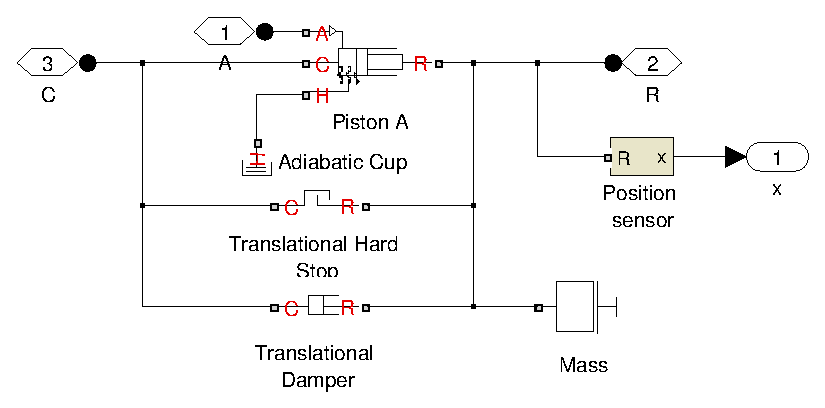
\includegraphics[scale=0.65]{implementation/figures/pneumatic_modelling3}
\caption{Simulink model of the pneumatic actuator.}
\label{fig:pneumatics_actuator}
\end{figure}

\subsubsection{Integrated Simulink Model}

The complete open-loop actuator model can be seen in Fig. \ref{fig:pneumatics_model_full}. The absolute value of the real-valued input $u$ is first fed to the PWM block. This signal is then converted into separate signals for each of the two solenoid valves in a way similar to the first PWM pulsing scheme presented by \citet{accurate_position}. The input to the subsystem $u$ is expected to range from -1 to 1. When $u\geq0$, the input to valve A is the pulse width modulated signal $U$, and the input to valve B is 0. When $u<0$, the opposite situation occurs.

\begin{figure}[H]
\centering
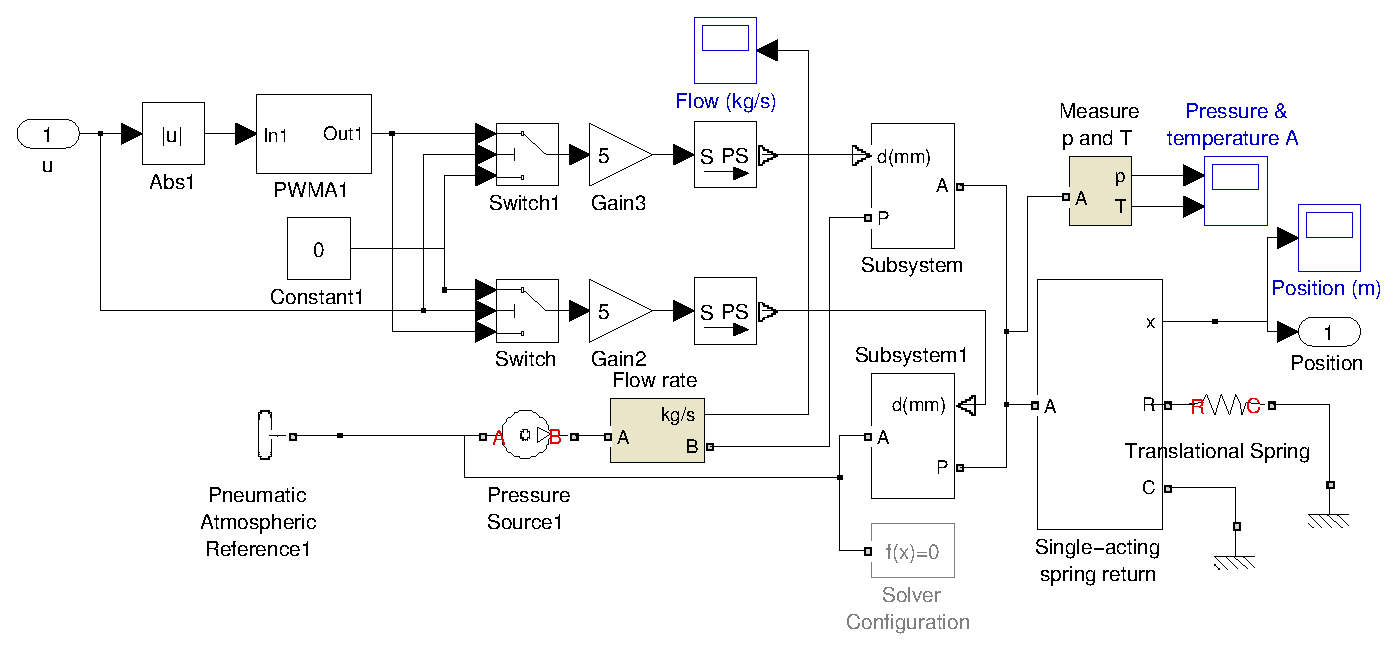
\includegraphics[scale=0.65]{implementation/figures/pneumatic_modelling4}
\caption{Simulink model of the full electro-pneumatic system.}
\label{fig:pneumatics_model_full}
\end{figure}

\subsection{Component Selection}

Selection of components was limited by budgetary constraints, however adequate solenoid valves and pneumatic actuators were found. These are detailed in the following sections.

\subsubsection{Solenoid Valves}

Solenoid valves and cylinders from SMC corp were chosen for the physical implementation of the design, specifically the \emph{VQZ115} series valve. Table \ref{tab:solenoid_specs} shows the specifications for this solenoid valve. A maximum operating frequency of \unit{20}{\hertz} was the fastest available solenoid that met the output force requirements while still being within the Formula SAE budget.

\begin{table}[H]
  \caption{Specifications of the SMC VQZ115 solenoid valve.\label{tab:solenoid_specs}}
  \centering

  \begin{tabular}{|l|l|}
  \hline
  Part & VQZ115-6L1-N1-PR \tabularnewline
  \hline
  Coil Voltage & \unit{12}{\volt} \tabularnewline
  \hline
  Configuration & 3-port Normally Closed \tabularnewline
  \hline
  Flow Coefficient & $C_v=\unit{0.23}{}$ \tabularnewline
  \hline
  Maximum Operating Frequency & \unit{20}{\hertz} \tabularnewline
  \hline
  Maximum Pressure & \unit{0.7}{\mega\pascal} \tabularnewline
  \hline
  \end{tabular}
\end{table}

\subsubsection{Pneumatic Actuators}

The pneumatic actuators specified for implementation are the same as used in the previous design, and are only briefly mentioned in this report. Specifications can be found in Table \ref{tab:cylinder_specs}. The clutch cylinder is specified with an internal magnet on the piston that interfaces magnetically with a membrane potentiometer, discussed next.

\begin{table}[H]
 \caption{Specifications of the pneumatic actuators used.\label{tab:cylinder_specs}}
  \centering
  \begin{tabular}{|l|l|l|l|}
   \hline
   Part & Bore Size & Stroke & Part Number \tabularnewline
    \hline
    \hline
    Shift actuator & 9/16`` & 2'' & NCMC056-0200 \tabularnewline
    \hline
    Clutch actuator & 3/4`` & 2'' & NCDMC075-0200 \tabularnewline
    \hline
  \end{tabular}
\end{table}

\subsubsection{Positional Feedback Sensors}

A ``MagnetoPot'' contact-less potentiometer from Spectra Symbal provides positional feedback from the clutch cylinder. The internal magnet in the cylinder interacts with the ``MagnetoPot'', which has a three-wire electrical interface similar to a standard potentiometer.

\section{Common Hardware Implementation\label{sec:common_hardware_implementation}}

In order to deliver high quality modules suitable for use in the vehicle, the module electronics were all implemented on custom designed two-layer printed circuit boards. Since the project budget could only afford the manufacture of a single iteration of prototype boards, a great deal of time was spent revising both the schematics and board layouts of all four modules to fix as many issues before sending them out for manufacture.

\nomenclature{PCB}{Printed Circuit Board}

\subsection{Base System Hardware\label{sec:base_system_hardware}}

All four modules are implemented on custom printed circuit boards (PCBs), and utilize a common base platform consisting of a microcontroller, a power supply, status leds, and JTAG programming header. Additionally, the telemetry, braking, and transmission and engine control modules utilize a special sealed 23-pin connector header.

Table \ref{tab:common_module_components} lists the major non-generic components that were specified as the common base for each module. An emph{AT90CAN128} micro-controller from Atmel was chosen for several reasons. We considered several simple, low cost microcontrollers specifically for automotive use as they are typically configured with the features we need, specifically, we wanted a microcontroller with:

\begin{itemize}
  \item a \unit{5}{\volt} power supply,
  \item integrated CANBus periferal,
  \item a large amount of on-chip RAM and ROM,
  \item in-circuit debugging and programming capabilities, and
  \item a flexible and cross-platform toolchain, ideally using GNU tools like gcc.
\end{itemize}

We considered the use of a 16-bit microcontroller, but felt it would be overkill for our system. The 8-bit AT90CAN128 met our requirements very well, and we had the additional benefit of already being somewhat familiar with the Atmel platform. The AT90CAN series runs off of a \unit{5}{\volt} power supply, has integrated CANBus, in addition to lots of other periferals \cite{AT90CAN}. The AT90CAN128 provides \unit{128}{\kilo\byte} ROM, however only \unit{4}{\kilo\byte} of RAM. We felt this would however suffice. The AT90CAN also supports a JTAG debugging interface, and there exists a very well developed open-source toolchain and standard c library, both of which will be described further in Sec. \ref{sec:common_software_implementation}.

\begin{table}[H]
	\caption{Common module components.}
	\label{tab:common_module_components}
	\centering
	\begin{tabular}{|c|c|c|}
		\hline 
		Part & Manufacturer & Part Number\tabularnewline 
		\hline \hline
		CAN Bus Transceiver & Microchip & MCP2551\tabularnewline \hline
		Microcontroller & Atmel & AT90CAN128\tabularnewline \hline
		Voltage Regulator & Linear Technology & LT1129CST5\tabularnewline		
		\hline
	\end{tabular}
\end{table}

\subsection{Inter-module Communication\label{sec:inter_module_communication}}

\nomenclature{CAN}{Controller Area Network}

All electronic systems on the vehicle communicate over a two-wire \emph{Controller Area Network} (CAN) bus operating at 1 MBit/s. Each system module has a Microchip-brand MCP2551 CAN transceiver IC for connecting their local micro-controller to the bus, and all modules are capable of being a termination point for the bus \cite{MCP2551}. The CAN transceiver electrically interfaces the microcontroller to the physical bus.

\subsection{Linear Regulator}

The LT1129 from Linear Technology was chosen as the \unit{5}{\volt} regulator because of several features it offers. The device is capable of supplying up to \unit{700}{\milli\ampere}, requires only a single \unit{3.3}{\micro\farad} output capacitor, accepts input voltages up to \unit{30}{\volt}, and has built-in thermal limiting \cite{LTC1129}.

\subsection{PCB Layout and CAD Design}

Schematic capture and PCB layout were both done using the free version of EagleCAD. Schematics and PCB layouts can be seen in Appendix \ref{cha:attached_dvd}. All four modules were layed out as two-layer PCBs with a groud plane on the bottom, and a VCC plane (\unit{+5}{\volt}) on the top. This aided routing, and reduced the possibility of ground loops since any connection to ground was as short as possible. For comparison with other figures showing the design and construction process of the modules, Fig.\ \ref{fig:driver_interface_layout} shows the board layout exported from Eagle CAD of the Telemetry module board. Layouts of the other three modules are available in Sec.\ \ref{cha:attached_dvd}. Where possible, surface mount components were selected to reduce the number of drills required in the PCB (and hence the cost).

\begin{figure}[h]
  \centering
  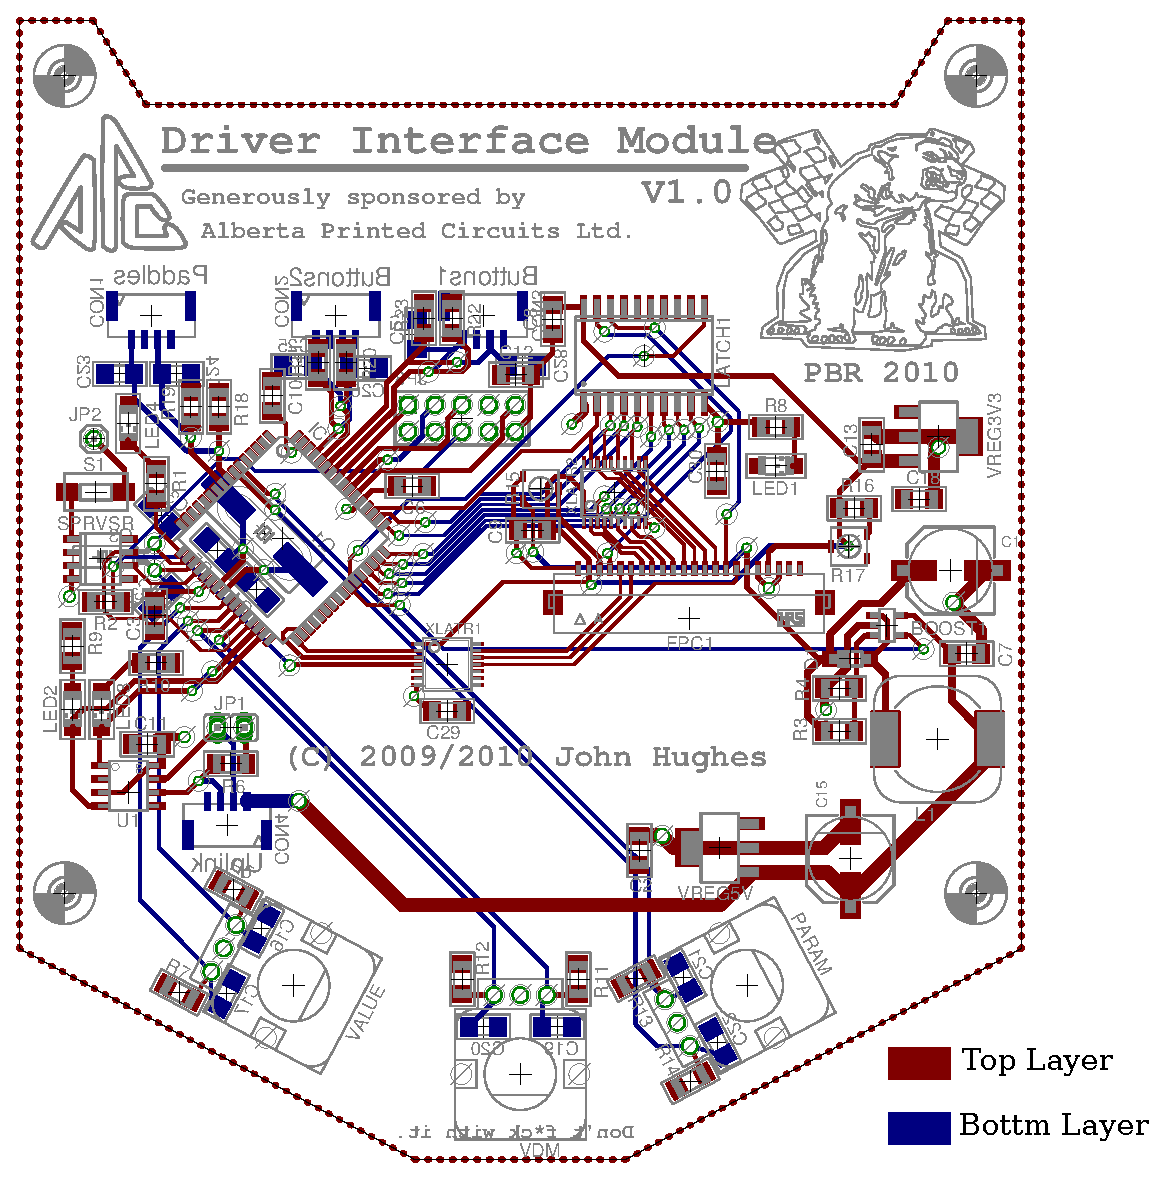
\includegraphics[width=3.5in,keepaspectratio]{implementation/figures/driver_interface_layout.eps}
  \caption{Board layout for the Telemetry module, exported from Eagle CAD.}
  \label{fig:driver_interface_layout}
\end{figure}

\subsection{Module Construction}

The printed circuit boards were manufactured by Alberta Printed Circuit (APCircuits), Ltd., who kindly sponsored the project. From the PCB layouts created in Eagle CAD, industry-standard GERBER-format files were generated and sent electronically to APCircuits. Figure \ref{fig:empty_pcbs} shows a photograph of the four empty PCBs after they were manufactured.

All four modules were populated and soldered by hand. Counter-intuitively, we found soldering the surface mount components with many leads to be easier than their through-hole counterparts. Initially we attempted to use paste stencils laser-cut out of mylar to apply the solder, in a process similar to that used in industry, however we found that for the relative incomplexity of our PCBs this was not of great aide. In the final manufacturing process, several steps were taken to populate each module:

\begin{enumerate}
  \item Once the circuit boards had arrived from manufacture, simple electrical tests were made to validate the construction: point to point checks of the ground and VCC planes were checked for continuity.
  \item An alchol-based circuit board cleaner was used to clean the surface of the boards of any contaminants.
  \item Solder paste was applied using a syringe individually to the large pads of resistors and capacitors, and in a thin strip across a line of smaller pads for the larger components.
  \item Individual components were placed on the pads with tweezers. The previously applied solder paste served as a slight adhesive.
  \item The entire board was placed in a toaster oven for approximately 7 minutes. Two-minute warm up and cool down periods were used before and after a 3 minute maximum tempurature reflow phase. The warm-up period served to evaporate the solvents in the solder paste, while the gradual cool down was performed to avoid thermal shock.
\end{enumerate}

\begin{figure}[h]
 \centering
 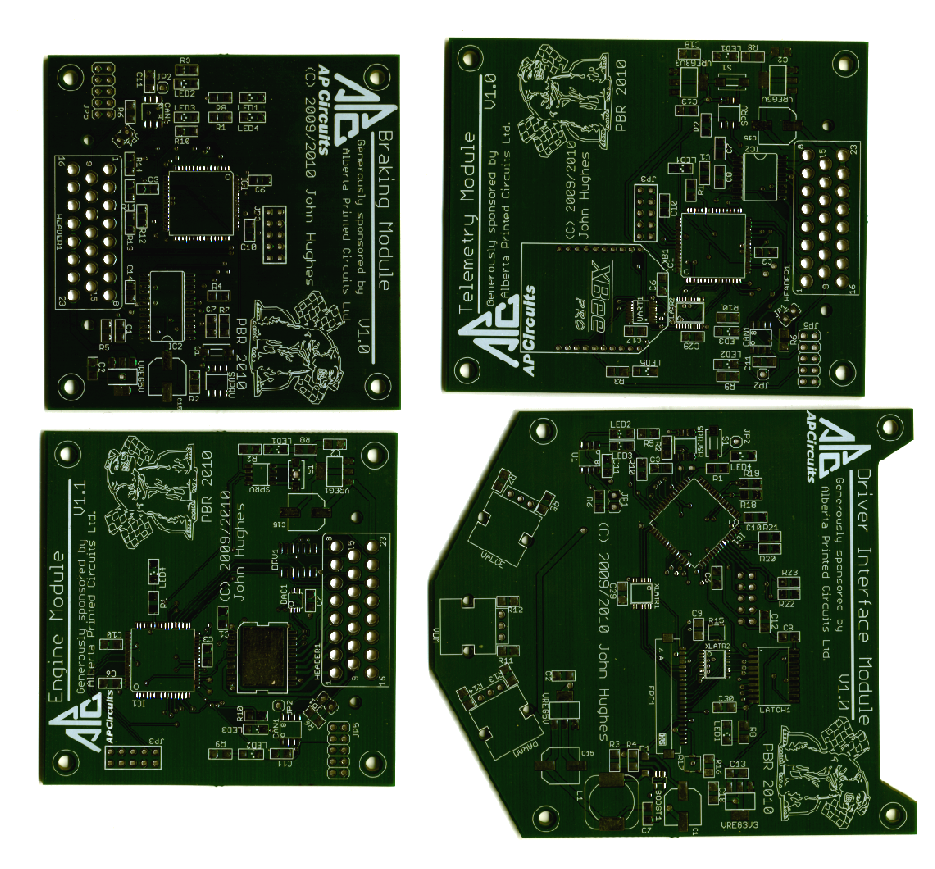
\includegraphics[width=5in,keepaspectratio]{implementation/figures/empty_pcbs.eps}
 \caption{Empty circuit boards after manufacturing. Clockwise: Braking module, Telemetry module, Driver Interface module, and Engine and Transmission module}
 \label{fig:empty_pcbs}
\end{figure}

Color photographs of each completed module are shown in the relevant sections discussing them.
\section{Common Software Implementation\label{sec:common_software_implementation}}

Hidden beneath the surface of the hardware is a substantial amount of system code written to implement the soft aspects of the design. In fact, thousands upon thousands of lines of code already exist. This section outlines the approach taken to control the complexity of the software, and details the tool-chain used. The hardware abstraction libraries shared by the four modules are also discussed.

\subsection{Methodology}
\label{sec:imp_software_meth}

Code re-usability was a primary target of the software implementation. However, this target was tempered by the need to write concise code that solves only problems that actually exist. Portability to other projects was not considered at all. Low-level hardware abstraction libraries for the various micro-controller peripherals were written as ``C'' libraries. These libraries are linked to module-specific code as needed. 

\nomenclature{RAM}{Random-Access Memory}

Because of the limited resources of the micro-controller, code efficiency was also of the utmost concern. The AT90CAN128 has \unit{4}{\kilo\byte} of \emph{random-access memory} (RAM). Data sizes were kept to a minimum, and buffers were also carefully managed. The use of dynamically allocated memory was avoided to reduce the possibility of memory leaks. The micro-controller features \unit{128}{\kilo\byte} of \emph{read-only memory} (ROM). Effort was made to place as much statically allocated data into the ROM as possible, such as string constants.

\subsection{Tool Chain}
\nomenclature{IDE}{Integrated Development Environment}

Atmel offers their own tool-chain and \emph{integrated development environment} (IDE) for Windows. Neither author uses Windows, but open-source support for the Atmel 8-bit micro-controllers is mature and capable. The development environment is documented in detail in Appendix \ref{apx:environment}.

\subsection{Hardware Abstraction Libraries}

As mentioned in Sec. \ref{sec:imp_software_meth}, several hardware abstraction libraries exist to simplify access to the peripherals of the micro-controller. These libraries are shared amongst the modules. 

\subsubsection{ADC Driver}

The ADC driver provides access to the on-board analog-to-digital converter hardware. The driver provides the ability to:

\begin{itemize}
	\item Sample any of the fifteen channels available to the ADC; 
	\item Operate in \emph{blocking} or \emph{non-blocking} modes; and
	\item Enable or disable the ADC to reduce power consumption.
\end{itemize}

In blocking mode, the micro-controller waits for the sampling process to complete before returning control to the program. In non-blocking mode, control returns back to the program immediately after the sampling begins. The user specifies a specific function to be called when sampling completes. 

\subsubsection{CAN Driver}
\label{sec:impl_can_driver}

The CAN driver provides a simplified interface to the functionality of the AT90CAN128's on-board CAN controller. The key features of the driver are:

\begin{itemize}
	\item Up to fifteen local \emph{message objects} available for sending and receiving;
	\item Support for CAN 2.0A and 2.0B identifier formats;
	\item The ability to assign receive and transmit \emph{callback functions} for each message object.
	\item An \emph{auto-reply} feature that listens for remote requests and replies with a pre-allocated data packet; and
	\item User-configurable baud-rate settings.
\end{itemize}

Users can configure message objects to receive or send a particular type of packet with any particular identifiers. The callback feature lets the user schedule functions to be executed whenever a message object receives or transmits a new packet. This allows asynchronous interaction with the bus and avoids wasteful polling strategies.

The auto-reply feature allows modules to automatically reply to incoming remote requests from particular identifiers. The data to be used for the reply can be udpated at any time, and the data must be flagged as ``valid'' by the user before transmission.

The driver is capable of operating at the standard CAN baud rates of 100, 125, 250, 500, and 1000 KBps. The baud rate is set at initialization time.

\subsubsection{EEPROM Driver}

The EEPROM driver provides a transparent interface to the 1024 bytes of EEPROM locates on the micro-controller. Writing data to the EEPROM is a relatively slow process that requires the micro-controller remain uninterrupted. The driver takes care of these details for the user. Specifically, the EEPROM driver implements:

\begin{itemize}
\item The ability to read and write 8-bit values to and from the EEPROM transparently; and
\item Protection against interruption during the write-process.
\end{itemize}

\subsubsection{SPI Driver}
\label{sec:impl_spi_driver}

The AT90CAN128 comes with a built-in SPI interface that generates the necessary signals required to communicate with SPI-capable devices. This interface is made available to the user through the SPI driver. Some aspects of the driver are:

\begin{itemize}
\item Single character and string based read and write functions; and
\item Dynamic configuration of up to eight slave select lines, including \emph{pin assignment} and \emph{transition delay}.
\end{itemize}

Up to eight slave select lines can be utilized by the driver. The user specifies which line is to be toggled at any given time. The user may also specify a delay (in microseconds) to be observed after transitioning the slave select lines. This allows the design to meet the varying timing requirements dictated by different SPI-enabled hardware.

\subsubsection{USART Driver}

The USART driver provides access to the receive and transmit functions of the AT90CAN128's built-in dual-channel USART. It also implements circular receive and transmit buffers to allow efficient data flow, and callback functions for asynchronously operation.
Some features of the USART driver are:

\begin{itemize}
	\item Two 64-byte circular receive and transmit buffers for each channel; and
	\item Callback functions for receiving and transmitting events.
\end{itemize}

The buffers have the ability to callback the user when particular events occur. These events include:

\begin{itemize}
\item A new byte has been received successfully; 
\item The receive buffer is full;
\item The receive buffer has overrun;
\item A new byte has been transmitted successfully; or
\item The transmit buffer is empty.
\end{itemize}

\section{Engine and Transmission Module}

\subsection{Hardware}

The engine and transmission module implements the design specified in Sec. \ref{sec:engine_transmission_design}.

In addition to the common life-support hardware for the micro-controller, the engine module includes an SPI capable octal \emph{low-side solenoid driver}. This driver chip switches the low side of the solenoid valves. It includes flyback protection circuitry to squash voltage spikes from the inductive load of the solenoid, and can also detect electrical shorts. 

\begin{figure}[H]
\centering
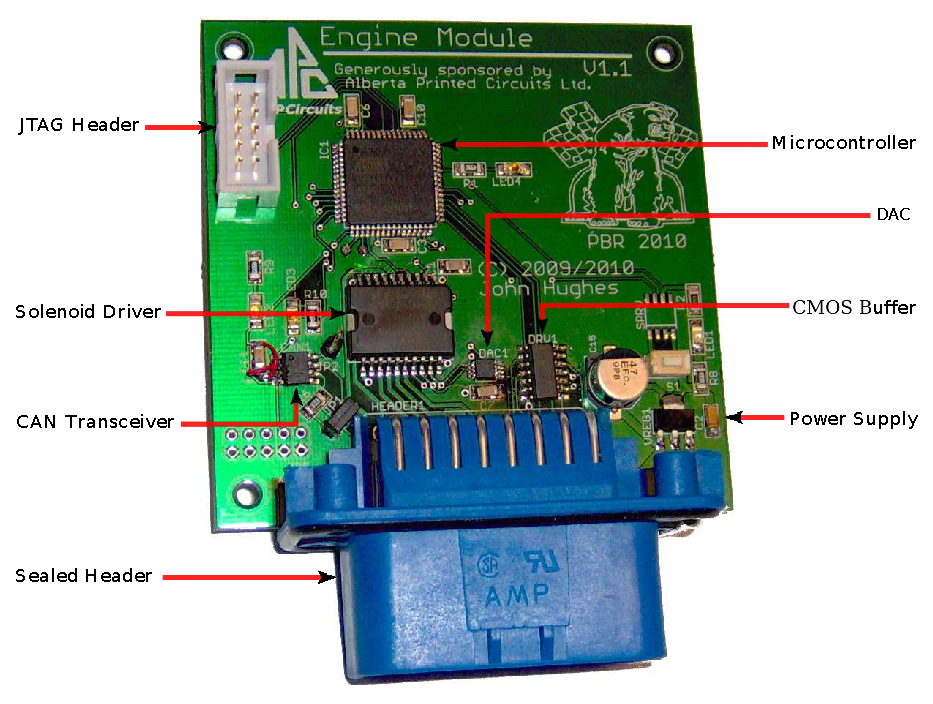
\includegraphics[scale=1]{implementation/figures/engine_transmission_pcb}
\caption{Populated Engine and Transmission module PCB.}
\label{fig:engine_transmission_pcb}
\end{figure}

\begin{figure}[H]
\centering
\begin{tikzpicture}[auto, node distance=3.5cm, draw=black!70, >=stealth']
  \node [block, name=at90] {AT90CAN};
  \node [block, name=dac, left of=at90] {TLV5623 DAC};
  \node [block, name=driver, right of=at90] {L9822E Solenoid Driver};
  \node [block, name=can, below of=at90, above=0.5cm] {MCP2551 CAN Transceiver};
  \node [block, name=buf, left of=can] {74LVC07 Buffer};

  \node [block, name=ecu, rotate=90, minimum width=8em] at ($(dac.west)!0.5!(buf.west)+(-1.25cm,0)$) {ECU};
  \node [block, name=solenoids, right of=driver, left=-0.75cm] {Solenoids};
  \node [block, name=feedback, below of=solenoids, above=0.75cm, text width=2.2cm, inner sep=0.05cm] {Position Transducers};

  \path (at90.north)+(0.0,+0.4) node (title) {Engine Module};

  \begin{pgfonlayer}{background}
    \path (dac.north west)+(-0.3,0.7) node (a) {};
    \path (can.south -| driver.east)+(+0.3,-0.2) node (b) {};
    \path[module] (a) rectangle (b);
  \end{pgfonlayer}

  \node [bus, name=can1, below of=can, label=below:CAN Bus, above=2.0cm] {CAN Bus};
  \node [bus, name=can2, left of=can1] {};
  \node [bus, name=can3, right of=can1] {};

  \draw [-, line width=3pt] (can) -- (can1);
  \draw [-, line width=3pt] (can1) -- (can2);
  \draw [-, line width=3pt] (can1) -- (can3);

  \draw [->, thick] (driver) -- (solenoids);

  \draw [->, thick] (at90) -- node[above] {SPI} (driver);
  \draw [<->, thick] (at90) -- (can);
  \draw [->, thick] (at90) -- node[above] {SPI} (dac);
  \draw [->, thick] ($(at90.west)+(0,-0.3)$) to[myncbar, arm=0.5cm, angle=180] (buf);
  \draw [<-, thick] ($(at90.east)+(0,-0.3)$) to[myncbar, arm=0.5cm] (feedback);

  \draw [->, thick] (dac.west) to[myncbar, arm=0.2cm, angle=180] ($(ecu.south)+(0,0.5)$);
  \draw [->, thick] (buf.west) to[myncbar, arm=0.2cm, angle=180] ($(ecu.south)+(0,-0.5)$);
% 
% 
%   \draw [-, line width=2pt] (can1) -- (can2);
%   \draw [-, line width=2pt] (can2) -- node[rotate=90, above] {CAN Bus} (can3);
%   \draw [-, line width=2pt] (can3) -- (can4);
% 
%   \node [bus, above of=can1, below=1cm] (tip1) {};
%   \node [bus, below of=can4, above=1cm] (tip2) {};
%   \draw [-, densely dashed, line width=2pt] (can1) -- (tip1);
%   \draw [-, densely dashed, line width=2pt] (can4) -- (tip2);
% 
%   \node [block, right of=can2, right, text width=8em] (engine) {Engine Module};
%   \node [block, right of=can3, right, text width=8em] (ecu) {ECU};
% 
%   \node [block, right of=engine, right, text width=8em] (starter) {Starter System};
%   \node [block, right of=ecu, right, text width=8em] (intake) {Intake System};
%   \node [block, above of=starter, text width=8em] (transmission) {Transmission System};
% 
%   \draw [<->] (engine) -- (ecu);
%   \draw [<->] (engine.south east) -- (intake.north west);
%   \draw [<->] (engine) -- (starter);
%   \draw [<->] (engine.north east) -- (transmission.south west);
% 
%   \draw [<->, line width=2pt] (can2) -- (engine);
%   \draw [<->, line width=2pt] (can3) -- (ecu);
\end{tikzpicture}
\caption{Engine and transmission module hardware overview.}
\label{fig:engine_system_overmview}
\end{figure}

\begin{table}
  \caption{Engine and Transmission module components.\label{table:engine_transmission_module_components}}
  \centering
  \begin{tabular}{|c|c|c|}
    \hline 
    Part & Manufacturer & Part Number\tabularnewline 
    \hline \hline
    Solenoid Driver & ST Microelectronics & L9822E \tabularnewline
    \hline
    Digital to Analogue Converter & Texas Instruments & TLV5623C \tabularnewline
    \hline
    Hex CMOS Buffer & Texas Instruments & 74LVC07A \tabularnewline
    \hline
  \end{tabular}
\end{table}


\subsubsection{High Current Solenoid Driver}

In order to meet the requirement of being able to energize the multiple solenoids specified in the design, an 8-way solenoid driver component from ST Microelectronics was chosen. The LT9822E provides a simple SPI interface for the microcontroller to talk to, and also takes care of possible flyback from the solenoids with built-in clamping diodes.

Using this single component strongly reduces the complexity of the output stage of the circuit, since multiple discrete high-current transistors were not needed.

\subsubsection{Input Buffers}


\subsubsection{Traction Control Analogue Output}

In order to generate a 0-5V analogue signal for the ECU's traction slip ratio input, as was described in Sec. \ref{sec:background_ecu_data_interfaces}, a simple SPI interfaced digital to analogue converter (DAC) from Texas Instruments was introduced. The TLV5623 outputs \unit{0-5}{\volt} analogue signal that varies with the digital input.

The output voltage from the DAC can be determined by the following equation:

\begin{equation}
V_{out}=2\cdot{V_{ref}}\,\frac{Code}{2^{n}}\,\volt
\end{equation}

where $V_{ref}$ is the reference voltage input to the chip, $n=8\,(bits)$, and $Code$ is the digital input value ranging from $0$ to $2^{n-1}$. Since we want to output $\unit{5}{\volt}$ at fullscale input,

\begin{equation}
2\cdot{V_{ref}}\,\frac{2^{7}}{2^{8}}=V_{ref}=\unit{5}{\volt}
\end{equation}.

The DC input resistance $R_{in}$ on the traction cut input pin on the ECU was measured using a series resistor with the input terminal to be $R_{in}\approx\unit{155}{\kilo\ohm}$. The output current of the DAC therefore will be at most $I_{out}=\frac{5v}{155k}\approx\unit{32.26}{\micro\ampere}$.

\subsection{Software}

<Software interface map>


\subsubsection{Transmission Manager}


\subsubsection{Intake Manager}


\subsubsection{Starter Manager}


\subsubsection{Event Scheduler}


\subsubsection{CAN Interface}

<Data flow diagram>


\subsubsection{PWM Generator}

An efficient method was devised to generate 2 synchronized PWM signals from the L9822E driver chip. The $32\, kHz$ external crystal was used as the input to the 8-bit TIM2 timer periferal on the microcontroller. The input to the timer was first scaled by 8 which provided a timebase:
\begin{equation}
TB=\frac{32.768\, kHz}{8}=4.096\, kHz
\end{equation}

The timebase period is then given by:
\begin{equation}
\frac{1}{TB}\approx244\,\mu{S}
\end{equation}

We then define a constant scaling factor for the PWM generator:
\begin{equation}
{PWM\_DUTY\_SCALE}=\frac{T_{PWM}}{TB}\approx205
\end{equation}

By loading the timers compare register with with a value scaled with the constant scaling factor, we can cause the timer to generate an interrupt precisely when a level change in the PWM is required.

When generating 2 waveforms with the same timer periferal, 8 combinations of duty cycles of channels A and B were identified, and can be seen in Figure \ref{fig:pwm_cases}.

Since the waveforms are synchronized, it can be seen that there are only 2 cases where 3 transitions per period are required, corresponding to \ref{fig:pwm_cases_1} and \ref{fig:pwm_cases_2}. This happens when both channels have $0<Duty<100\%$. 2 cases are also apparent when no transitions are required, shown in \ref{fig:pwm_cases_7} and \ref{fig:pwm_cases_8}.

An efficient generating routine was constructed to effect the level transitions and to reset the timer to interrupt at the next transition. For the two cases requiring 3 transitions per period, the timer interrupts 3 times per period. For the two cases where both channels have duty cycle between 0 and 100\%, the routine still interrupts once to allow for a change in duty cycle. For the rest of the cases described, the timer only interrupts twice per PWM period.

\begin{figure}[ht]
  \centering
  \subfigure[Case 1]
  {
    \label{fig:pwm_cases_1}
    \begin{tikztimingtable}
      $PWM_A$		& G 4H 4L \\
      $PWM_B$		& G 2H 6L \\
    \end{tikztimingtable}
  }
  \subfigure[Case 2]
  {
  \label{fig:pwm_cases_2}
  \begin{tikztimingtable}
    $PWM_A$		& G 4H 4L \\
    $PWM_B$		& G 6H 2L \\
  \end{tikztimingtable}
  }
  \subfigure[Case 3]
  {
  \label{fig:pwm_cases_3}
  \begin{tikztimingtable}
    $PWM_A$		& G 4H 4L \\
    $PWM_B$		& 8L \\
  \end{tikztimingtable}
  }
  \subfigure[Case 4]
  {
  \label{fig:pwm_cases_4}
  \begin{tikztimingtable}
    $PWM_A$		& G 4H 4L \\
    $PWM_B$		& G 8H G \\
  \end{tikztimingtable}
  }
  \subfigure[Case 5]
  {
  \label{fig:pwm_cases_5}
  \begin{tikztimingtable}
    $PWM_A$		& G 8H G \\
    $PWM_B$		& G 4H 4L \\
  \end{tikztimingtable}
  }
  \subfigure[Case 6]
  {
  \label{fig:pwm_cases_6}
  \begin{tikztimingtable}
    $PWM_A$		& 8L \\
    $PWM_B$		& G 4H 4L \\
  \end{tikztimingtable}
  }
  \subfigure[Case 7]
  {
  \label{fig:pwm_cases_7}
  \begin{tikztimingtable}
    $PWM_A$		& 8L \\
    $PWM_B$		& 8L \\
  \end{tikztimingtable}
  }
  \subfigure[Case 8]
  {
  \label{fig:pwm_cases_8}
  \begin{tikztimingtable}
    $PWM_A$		& G 8H G \\
    $PWM_B$		& G 8H G \\
  \end{tikztimingtable}
  }
  \caption{PWM Cases (1 period shown).}
  \label{fig:pwm_cases}
\end{figure}

\subsubsection{Main Control Loop}
\section{Braking Module}

The Braking module implements the design specified in Sec.\ \ref{sec:Braking-Module-Design}. The hardware and software aspects of this module's implementation are discussed in this section.

\begin{figure}[h]
\centering
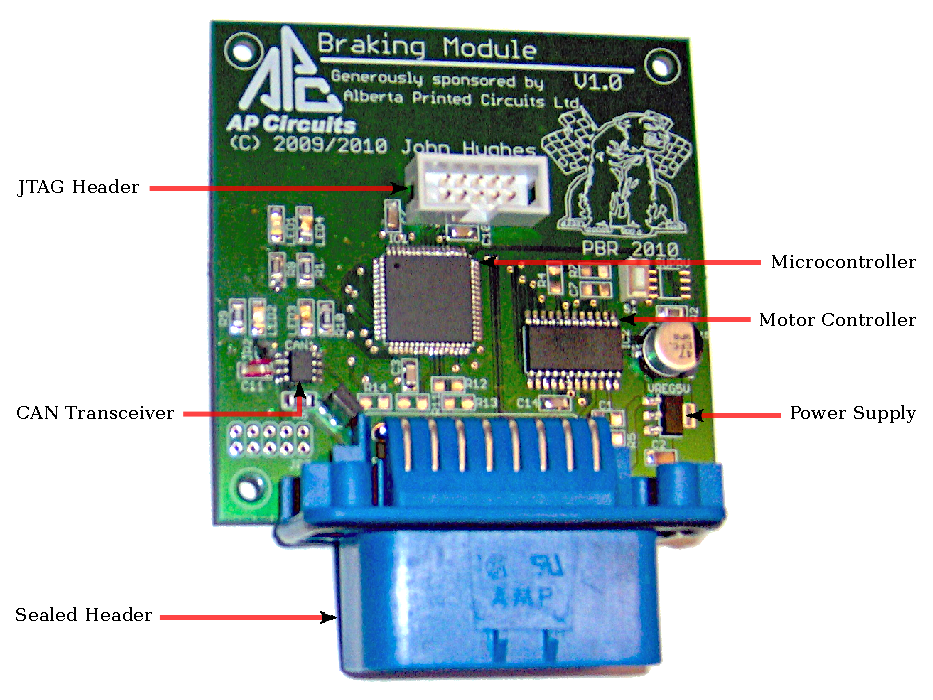
\includegraphics[scale=1]{implementation/figures/braking_pcb}
\caption{Populated Braking module PCB.}
\label{fig:braking_pcb}
\end{figure}

\subsection{Hardware}

The braking module implementation was the simplest of the 4 modules in terms of electrical design. Only one special hardware component was required, namely the stepper motor driver. This is summarized in Table \ref{table:braking_module_components}.

Figure \ref{fig:braking_pcb} shows a photograph of the completed braking module circuit board, with all components soldered on. The simplicity of the electrical design is reflected in the fact that no additional corrections (other than for the CAN transceiver) were required for the module to be 100\% operational.

\begin{table}
  \caption{Braking module components.\label{table:braking_module_components}}
  \centering
  \begin{tabular}{|c|c|c|}
    \hline 
    Part & Manufacturer & Part Number\tabularnewline 
    \hline \hline
    Stepper Motor Controller/Driver & Allegro Microsystems & A3967 \tabularnewline
    \hline
  \end{tabular}
\end{table}

\subsubsection{Stepper Motor Driver}

In order to meet the design goal of having the implementation be flexible in terms of which stepper motor would be used in the system, a current-sensing stepper motor controller/driver component was used in the circuit design. The current sense capability allows us to fix the input voltage in the circuit design, and afterwards adjust the current drive by changing resistor values in the current-sense feedback loop. 

The A3967 ``Micro-stepping Driver with Translator'' was chosen to drive the stepper motor for several reasons. The A3967 integrates a micro-stepping controller with dual H-Bridge output stages into one package. This simplified the potential circuit design. The H-Bridge output transistors can supply up to $\pm\unit{750}{\milli\ampere}$ of current at up to \unit{30}{\volt} \cite{A3967}. 

\paragraph{Current Control}
\nomenclature{$R_{sense}$}{Value of the current sense resistors in the Braking Module's stepper motor circuit.}
\nomenclature{$I_{TRIP}max$}{Maximum current allowed to flow into the Braking Module's stepper motor before the PWM circuit shuts the output stage off.}

The current control feature of the A3967 works by sensing the current through a sense resistor, $R_{sense}$, and varies the duty cycle of a fixed off-time PWM circuit, which controls the output from the H-Bridge stages.

The value of the sense resistor was determined by an equation recommended in the datasheet:
\begin{equation}
R_{sense}=\frac{0.5}{I_{TRIP}max}
\end{equation}
where $I_{TRIP}max$ is the maximum current allowed to flow into the motor before the PWM circuit shuts the output stage off.

The actual value of $R_{sense}$ used for bench testing the Braking module was \unit{2}{\ohm}, which allows \unit{250}{\milli\ampere} output current. This was suitable for the stepper motor used in testing.

\subsubsection{Analogue-to-Digital Converter}

The AT90CAN128's built-in analogue-to-digital converter was used to measure the analogue signals from the brake pressure transducers.

\subsubsection{End-of-Travel Microswitches}



\subsection{Software}


\subsubsection{Bias Library}


\paragraph{Bias Position Request}

<Position request flow chart>


\paragraph{Bias Calibration}

<Calibration flow chart>


\subsubsection{Pressure Library}


\paragraph{Periodic Pressure Output}


\paragraph{Pressure Calibration}

<Calibration flow chart>


\subsubsection{CAN Interface}

<Data flow diagram>


\subsubsection{Main Control Loop}
\section{Telemetry Module}

The telemetry module implements the design specified in Sec.\ \ref{sec:Telemetry-Module-Design}. The hardware and software aspects of this module's implementation are discussed in this section. Figure \ref{fig:telemetry_pcb} shows a photo of the completely populated and debugged telemetry module hardware.

\begin{figure}[H]
\centering
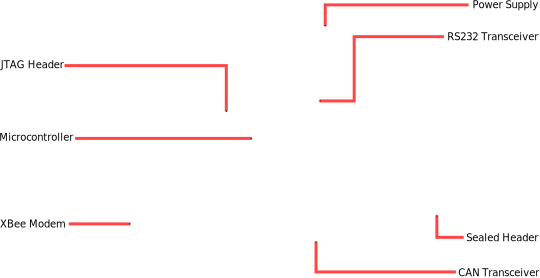
\includegraphics[scale=1]{implementation/figures/telemetry_pcb.eps}
\caption{Populated telemetry module PCB.}\label{fig:telemetry_pcb}
\end{figure}

\subsection{Hardware}

In addition to the base system hardware common to all modules described in Sec.\ \ref{sec:base_system_hardware}, several additional components were required in the implementation of the telemetry module. A block diagram of the telemetry module hardware implementation is shown in Fig.\ \ref{fig:telemetry_hardware_block}. The additional components are an XBee-PRO wireless mode, MAX232 RS-232 transceiver, MAX3100 external UART, an LTI1521 \unit{3.3}{\volt} linear voltage regulator, and an ST2378E 8-bit level translator. These additional components are listed in Table \ref{tab:telemetry_module_components} and will be described further in this chapter.

\begin{figure}[H]
\centering
\def\antenna{
  -- +(0mm,4.0mm) -- +(2.625mm,7.5mm) -- +(-2.625mm,7.5mm) -- +(0mm,4.0mm)
}

\begin{tikzpicture}[auto, node distance=4cm, draw=black!70, >=stealth']
  \node [block, name=max3100] {Max3100 SPI UART};
  \node [block, name=at90, right of=max3100] {AT90CAN};
  \node [block, name=rs232, right of=at90] {Max232 RS232 Transceiver};
  
  \node [block, name=can, below of=at90, above=1cm] {MCP2551 CAN Transceiver};
  \node [block, name=modem, left of=can] {XBee Modem};
  
  \node [block, name=ecu, right of=rs232] {ECU};
  \node [block, name=dac, below of=ecu, above=1cm] {DAC};

  \path (at90.north)+(0.0,+0.4) node (title) {Telemetry Module};

   \begin{pgfonlayer}{background}
       \path (max3100.north west)+(-0.3,0.7) node (a) {};
       \path (can.south -| rs232.east)+(+0.3,-0.2) node (b) {};
       \path[module] (a) rectangle (b);
   \end{pgfonlayer}

  \node [bus, name=can1, below of=can, label=below:CAN Bus, above=2.5cm] {CAN Bus};
  \node [bus, name=can2, left of=can1] {};
  \node [bus, name=can3, right of=can1] {};

  \draw [-, thick] (modem.west) -| ($(modem.west)+(-0.8,0.2)$) \antenna;

  \draw [-, line width=3pt] (can) -- (can1);
  \draw [-, line width=3pt] (can1) -- (can2);
  \draw [-, line width=3pt] (can1) -- (can3);

  \draw [<->, thick] (at90) -- node[] {SPI} (max3100);
  \draw [<->, thick] (max3100) -- node[text width=2cm] {Serial} (modem);
  \draw [<->, thick] ($(at90.east)+(0,0.1)$) to[myncbar, arm=1cm] ($(rs232.north west)+(0,-0.5)$);
  \draw [<-, thick] ($(at90.east)+(0,-0.1)$) to[myncbar, arm=1cm] ($(rs232.south west)+(0,+0.5)$);

  \draw [<->, thick] ($(rs232.north east)+(0,-0.5)$) to[myncbar, arm=1cm] (ecu);
  \draw [<-, thick] ($(rs232.south east)+(0,0.5)$) to[myncbar, arm=1cm] (dac);

  \draw [<->, thick] (at90) -- (can);

%  \draw [<->, thick] (modem) -- node[] {} (telemetry);
%  \draw [<->, thick] (telemetry) -- node[] {RS232} (ecu);
%  \draw [<->, thick] (telemetry) -- node[] {RS232} (daq);
%  \draw [-, thick] (modem) -- node[text width=1.5cm] {} (ant) \antenna;
\end{tikzpicture}
\caption{Telemetry module hardware block diagram.\label{fig:telemetry_hardware_block}}
\end{figure}

\begin{table}[H]
  \caption{Telemetry module components\label{tab:telmetry_module_components}}
  \centering
    \begin{tabular}{|c|c|c|}
      \hline 
      Part & Manufacturer & Part Number\tabularnewline
      \hline
      \hline
      XBee-PRO OEM Module & Digi International & XBee-PRO\tabularnewline
      \hline 
      Dual RS-232 Transceiver & Maxim Electronics & MAX232\tabularnewline
      \hline 
      SPI-capable UART chip & Maxim Electronics & MAX3100\tabularnewline
      \hline 
      300mA Low Dropout Regulator & Linear Technology & LT1521\tabularnewline
      \hline
      8-bit dual-supply level translator & ST Microelectronics & ST2378E\tabularnewline
      \hline
    \end{tabular}
\end{table}

\subsubsection{Dual RS-232 Transceiver}

The ECU and the DAQ modules connect to the telemetry board with specialized cables that connect to the wiring harness. The ECU and DAQ interface with two built-in USART ports on the AT90CAN128 micro-controller. A MAX232 dual RS-232 trasceiver chip was used in the design to interface the built-in UARTS on the AT90CAN128 with the line levels expected by the serial ports on the ECU and DAQ.

\subsubsection{XBee-PRO Wireless Modem and External SPI UART}

To meet the range and data throughput requirements for the telemetry system, an XBee-PRO wireles modem was used. The XBee requires \unit{3.3}{\volt} I/O levels and power supply, and so a second linear voltage regulator was used in the design, the LT1521 from Linear Technology. Since the AT90CAN129 has only 2 built-in UARTS that were used for the RS232 interfaces to the ECU and DAQ, an third external UART was added to the design. The MAX3100 is a SPI-interfaced UART with an 8 word deep FIFO buffer. It is interfaced to the AT90CAN128's SPI pins and has an active-low IRQ line connected to external interrupt line EXT7 on the microcontroller.

The wireless transmitter consumes at most \unit{215}{\milli\ampere} of current during transmit \cite{XBeeManual}. Since the common module hardware only provides power for 5V devices, the telemetry module has a second LDO regulator providing \unit{3.3}{\volt}. A separate antenna port is connected to the modem and mounted in the side of the module enclosure.

Since the XBee, MAX3100, and AT90CAN128 are operating at different logic levels, a dual-supply level translator was used. Signals between the XBee, MAX3100, and the low supply voltage side of the level translator use \unit{+3.3}{\volt} logic, while signals between the AT90CAN128 and the high supply voltage side of the level translator use \unit{+5}{\volt} logic.

\subsection{Software}

The primary objective of the software running on the telemetry module is to push data around from various sources to various sinks. An overview of the telemetry module's system software can be seen in Fig.\ \ref{fig:telemetry_software_implementation}. A layer of software drivers interacts directly with the hardware, providing an easy-to-use interface for the specific system software to use. Interrupt-driven USART drivers were written for the on-board USARTs of the AT90CAN128, as well as the MAX3100 external UART.

Three major libraries 

Nearly 3000 lines of c code were written by us for the telemetry modules' system software. 3800 lines of code were also contributed by David Schilling for the DAC library.

\begin{figure}[H]
\centering
\begin{tikzpicture}[auto, node distance=2cm, draw=black!70, >=stealth']
%  \draw[help lines] (-3,-5) grid (8,2);
  
  % Usart0 section
  \node [blue shiny, rectangle, minimum width=2cm] (usart0) {UART0};
  \node [blue shiny, rectangle, above of=usart0, node distance=1cm] (ecu) {ECU};

  \node [red shiny, rectangle, below of=usart0, right=-1cm, node distance=1cm] (usart0_rx) {Rx};
  \node [red shiny, rectangle, below of=usart0, left=-1cm, node distance=1cm] (usart0_tx) {Tx};

  \draw [<->] (ecu) to (usart0);
  \draw [<-] (usart0_rx) -- ($(usart0.south west)!(usart0_rx.north)!(usart0.south east)$);
  \draw [->] (usart0_tx) -- ($(usart0.south west)!(usart0_tx.north)!(usart0.south east)$);
  
  % Max3100 section
  \node [blue shiny, rectangle, minimum width=2cm, right of=usart0, node distance=3cm] (max3100) {MAX3100};
  \node [blue shiny, rectangle, above of=max3100, node distance=1cm] (xbee) {Xbee};
  \node [blue shiny, rectangle, below of=max3100, above=-0.3cm, left=0.25cm, node distance=0, font=\tiny, inner sep=0.075cm] (max3100_rx_hw) {Rx};

  \node [red shiny, rectangle, below of=max3100, right=-1cm, node distance=1cm] (max3100_rx) {Rx};
  \node [red shiny, rectangle, below of=max3100, left=-1cm, node distance=1cm] (max3100_tx) {Tx};

  \draw [<->] (xbee) to (max3100);
  \draw [<-] (max3100_rx) -- ($(max3100_rx_hw.south west)!(max3100_rx.north)!(max3100_rx_hw.south east)$);
  \draw [->] (max3100_tx) -- ($(max3100.south west)!(max3100_tx.north)!(max3100.south east)$);

  \node [red shiny, rectangle split, rectangle split parts=3, below of=max3100, text width=1.8cm, font=\scriptsize, text centered,
	  minimum width=2cm, anchor=base] (xbee_library)
    {XBee Library
      \nodepart{second} Packetizer
      \nodepart{third} Packet Buffer};

  %\node [red shiny, rectangle, below of=packetizer, node distance=1cm, minimum width=2cm,
%	  text width=1.75cm, font=\scriptsize, text centered] (packet_buf) {Rx Packet Buffer};

  \draw [->] (max3100_rx) -- ($(xbee_library.north west)!(max3100_rx.south)!(xbee_library.north east)$);
  \draw [<-] (max3100_tx) -- ($(xbee_library.north west)!(max3100_tx.south)!(xbee_library.north east)$);

  % Usart1 section
  \node [blue shiny, rectangle, minimum width=2cm, right of=max3100, node distance=3cm] (usart1) {UART1};
  \node [blue shiny, rectangle, above of=usart1, node distance=1cm] (dac) {DAC};

  \node [red shiny, rectangle, below of=usart1, right=-1cm, node distance=1cm] (usart1_rx) {Rx};
  \node [red shiny, rectangle, below of=usart1, left=-1cm, node distance=1cm, dashed] (usart1_tx) {Tx};

  \draw [<->] (dac) to (usart1);
  \draw [<-] (usart1_rx) -- ($(usart1.south west)!(usart1_rx.north)!(usart1.south east)$);
  \draw [->, dashed] (usart1_tx) -- ($(usart1.south west)!(usart1_tx.north)!(usart1.south east)$);

  \node [red shiny, rectangle split, rectangle split parts=4, below of=usart1, text centered, minimum width=2cm, anchor=base, text width=1.85cm, inner xsep=0, font=\scriptsize] (dac_library)
    {DAC Library
      \nodepart{second} Buffer
      \nodepart{third} Decoder
      \nodepart{fourth} Encoder};

  \draw [->] (usart1_rx) -- ($(dac_library.north west)!(usart1_rx.south)!(dac_library.north east)$);
  \draw [<-, dashed] (usart1_tx) -- ($(dac_library.north west)!(usart1_tx.south)!(dac_library.north east)$);

  % CAN stuff
  \node [blue shiny, rectangle, minimum width=2cm, right of=usart1, node distance=3cm] (can) {CAN};
  \node [red shiny, rectangle, minimum width=2cm, below of=can, node distance=1cm] (can_driver) {Driver};

  \node at (dac_library.third split -| can_driver)
	    [red shiny, rectangle, minimum width=2cm, text width=1.85cm, font=\scriptsize, text centered] (can_library) {Telemetry CAN Library};

  \draw [<->] (can) -- (can_driver);
  \draw [<->] (can_driver) -- (can_library);

  \draw [->] (dac_library.third east) -- ($(can_library.north west)!(dac_library.third east)!(can_library.south west)$);
  \draw [<-] (dac_library.fourth east) -- ($(can_library.north west)!(dac_library.fourth east)!(can_library.south west)$);

  % Now for the rest of the connections
  \draw [->] (xbee_library.third west) -| (usart0_tx);
  \draw [<-] (xbee_library.second west) -| (usart0_rx);
  \draw [->] (dac_library.second west) to node [name=mid1] {} (xbee_library.second east);
  \draw [->] (dac_library.fourth west) -| (mid1);

  \node [left of=usart0, node distance=3cm, minimum width=3.5cm] (perifs) {Module Periferals};
  \node [below of=perifs, node distance=1cm, minimum width=3.5cm] (buffers) {Drivers/Buffers};
  \node [below of=buffers, node distance=1cm, minimum width=3.5cm] (libraries) {Libraries};

  \begin{pgfonlayer}{background}
    \path (perifs.north west)+(-0.0,0.1) node (a1) {};
    \path (can.south east)+(+0.1,-0.1) node (b1) {};
    \path[draw=blue!50!black!50, rounded corners=0.1cm] (a1) rectangle (b1);

    \path (buffers.north west)+(-0.0,0.1) node (a2) {};
    \path (can_driver.south east)+(0.1,-0.1) node (b2) {};
    \path [draw=red!50!black!50, rounded corners=0.1cm] (a2) rectangle (b2);

    \path (libraries.north west)+(-0.0,0.1) node (a3) {};
    \path (can_library.south east)+(0.1,-0.1) node (b3) {};
    \path [draw=red!50!black!50, rounded corners=0.1cm] (a3) rectangle (b3);
  \end{pgfonlayer}

  % Guide
  \node at ($(a3 |- b3)+(0.0,-0.1)$) [anchor=north west, blue shiny, minimum width=2cm] (hardware) {Hardware};
  \node [red shiny, right of=hardware, node distance=2.2cm, minimum width=2cm] (software) {Software};
  
\end{tikzpicture}

\caption{Telemetry module software overview.}
\label{fig:telemetry_software_implementation}
\end{figure}

\subsubsection{MAX3100 External UART Driver}

The software driver written for the MAX3100 exteran UART was crafted in the image of the built-in USART driver, and shares the same software interfaces and buffering code. The drivers was written to utilize the external hardware interrupt to allow asynchronous sending and receiving of data. A statically allocated circular buffering approach was taken for both receiving and transmitting data. An abstracted flow chart of the interrupt handling is shown in Fig.\ \ref{fig:usart_driver_flow}.

The datahseet for the MAX3100 states that the minimum SPI Clock period is $t_{CP}=\unit{238}{\nano\second}$, which results in a maximum frequency of approximately $\unit{4.2}{\mega\hertz}$ \cite{MAX3100}. The SPI periferal was thus set to use 1/4 of the system clocks frequency when communicating with the MAX3100, resulting in $\unit{4}{\mega\hertz}$ SPI clock speed.

\begin{figure}[H]
\centering
\begin{tikzpicture}[auto, node distance=2cm, draw=black!70, >=stealth']
  \node [start] (int) {Interrupt};
  \node [decision, right of=int, right=0cm] (rx) {Rx Byte?};
  \node [block, below of=rx] (add) {Add to Rx buf.};

  \node [decision, right of=rx, right=0cm] (tx) {Tx Byte?};
  \node [block, below of=tx, text width=2.5cm, inner xsep=0pt] (remove) {Remove from Tx buf.};
  \node [end, right of=tx, right=0cm] (return) {Return};

  \draw [->] (int) -- (rx);
  \draw [->] (rx) to node [] {yes} (add);

  \draw [->] (rx) -- node [name=mid] {no} (tx);
  \draw [->] (add) -| (mid);

  \draw [->] (tx) to node [] {yes} (remove);
  \draw [->] (tx) -- node [name=mid2] {no} (return);
  \draw [->] (remove) -| (mid2);

\end{tikzpicture}
\caption{Basic USART interrupt flow diagram.}
\label{fig:usart_driver_flow}
\end{figure}

\subsubsection{XBee Library}

In order to facilitate routing data to and from multiple sources and sinks, it was determined that the XBee would need to be interfaced using the special ``API'' mode described in the XBee documentation \cite{XBeeManual}. The API mode is characterized by a packet interface that would require a supporting library in software. The library was written to implement two critical pieces of functionality:

\begin{enumerate}
\item and to send and receive packetized data from the modem on behalf of the user software as per the XBee's API specification \cite{XBeeManual};
\item to set the modem into API mode operation and manage the modem's operating state;
\end{enumerate}

The XBee library can be split logically into two chunks: code to packetize outgoing data for the main control loop software, and code to disassemble incoming packets and provide their payload to the main control loop.

The XBee library implements the binary packet protocol described in the XBee manual, and is able to send and receive unicast and multicast packets. The driver is only capable of sending packets to 16-bit addresses. Full 64-bit address mode was not implemented as the address space was not required in our 3 node network. The driver is also capable of sending command-type packets to the modem and reading the response.

When the mainline software wants to send a packet, it calls the \verb|xbee_send_data()| function. A pointer to the data as well as the 16-bit address is passed. The packet is constructed, and the packetized data is added to the MAX3100 driver's TX buffer to be sent to the XBee.

Receiving packets is more complicated, since individual bytes arrive at the MAX3100 drivers's RX buffer asynchronously. A state machine was constructed that waits for a full packet to be available in the RX buffer, and then pushes it into a seperate, incoming packet buffer. This incoming packet buffer can then be read by the mainline code.

Managing the modem's state was implemented as a state machine. Since minimal functionality was required, only a handful of modem commands were implemented. The driver is able to push the modem into API mode, after which all communication is done using the packet interface. The modem commands implemented by the telemetry module are listed in Table \ref{tab:xbee_commands}.

\begin{table}
\caption{Implemented XBee modem commands.\label{tab:xbee_commands}}
\centering{}
\begin{tabular}{|l|l|}
\hline 
Command & Description \tabularnewline
\hline
\hline
AP & Set and read the API mode state \tabularnewline
\hline
CH & Set and read the RF channel \tabularnewline
\hline 
ID & Set and read the PAN (Personal Area Network) ID \tabularnewline
\hline
MY & Set and read the modems local address \tabularnewline
\hline
\end{tabular}
\end{table}

The XBee modem can be controlled out of API mode by entering into it's command mode by sending a special string of bytes, by default ``+++''. A list of modem-style AT-commands, documented in the manual, are used to change the various settings of the modem. This command mode was used to initially set up the modems by hand, but is only used by the software once on startup to enable the API mode.

Similar to the rest of the software drivers implemented, the XBee library uses callbacks to provide the user software with incoming data. Function pointers are used to connect the library to a UART, which makes it possible to reconfigure the library to use a different USART on-the-fly.

\subsubsection{DAC Library\label{sec:dac_library}}

To reduce the implementation work required by us, we asked David Schilling, a computer science student on the Formula SAE team, to write the DAC software library to read and write the DAC's serial format, given the requirements described in Section \ref{sec:Telemetry-Module-Design}.

The DAC library maintains it's own buffer of incoming DAC data. We also asked Dave to provide seperate functions for buffering incoming data, and for processing that data. This seperation allowed the library to be easily tied in with the rest of the system software on the telemetry module: adding data to the DAC buffer occurs whenever the internal USART driver interrupts with a new byte, and processing is called from the mainline loop.

Transmission of DAC data over the wireless link is synchronized with the DAC Libraries' decoder. Whenever an entire DAC packet is decoded by the library, that packet is then sent in it's entirety over the link. Since transmission is done packet-wise, and not byte-by-byte, the injection of arbitrary packets into the DAC serial stream is possible without having packets collide.

\subsubsection{Main Control Loop}

Once all of the hardware on the module is initialized and the XBee has successfully entered API mode, the telemetry module's main control loop repeatedly calls the \verb|telemetry_process()| function. This function runs through three seperate processes:
\begin{enumerate}
  \item The RX buffer of the USART that the ECU is connected to is polled for data. If there is any incoming data waiting, send it over the ECU link by passing it to the packetizer;
  \item all decoded packets in the incoming packet buffer are dealt with, by calling\\ \verb|xbee_digest_incoming_packets()|;
  \item and finally, an iteration of the DAC libraries' decoder function is called,\\ \verb|dac_decode_serial()|. This checks to see if any of the buffered incoming DAC data can be decoded.
\end{enumerate}

Incoming DAC data does not need to be polled in the same way as with the ECU, since an incoming byte callback is set which places any incoming DAC bytes into the DAC libraries' own buffer.
\section{Driver Interface Module}

The Driver Interface module implements the design specified in Sec.\ \ref{sec:Driver-Interface-Module}. The hardware and software aspects of this module's implementation are discussed in this section. Figure \ref{fig:driver_interface_pcb} shows a photo of the completely populated and debugged Driver Interface module hardware.

\begin{figure}[h]
\centering
\includegraphics[scale=1]{implementation/figures/driver_interface_pcb.eps}
\caption{Populated telemetry module PCB.}\label{fig:driver_interface_pcb}
\end{figure}

\subsection{Hardware}

In addition to the base system hardware common to all modules described in Sec.\ \ref{sec:base_system_hardware}, the Driver Interface module provides all of the support hardware needed for the LCD module to function. An FPC connector, LCD bias boost converter, \unit{+3.3}{\volt} power supply, latch for the interface to the microcontroller, as well as level translators to translate from the microcontroller's \unit{+5}{\volt} logic to the LCD Controller's \unit{+3.3}{\volt} logic are all included in the module. Additionally, 3 rotary encoders are soldered on the board. On the back of the PCB are connectors to the steering wheel-mounted push buttons and paddles.

The LCD module used in the Driver Interface implementation is a packaged LCD module from Newhaven Display. Along with the actual LCD panel, a built-in display controller chip and display RAM are included. Interfacing with the LCD module entails interfacing with it's controller chip, a SED1335 LCD controller IC from Seiko Epson Corporation. The controller chip handles all of the low level functionality of the LCD, such as generating pixel clocks and drawing to the screen from the LCD RAM. It also provides a character generator.

\subsubsection{LCD Module Bias Circuit}

According to the datasheet, the LCD screen requires a large bias voltage of \unit{+22}{\volt} \cite{LCD_Module}. A Linear Technology LT1615 step-up DC/DC converter was chosen as the centre of a boost converter circuit to generate the bias voltage, shown in Fig.\ \ref{fig:lcd_boost_converter}.

\begin{figure}[htp]
 \centering
 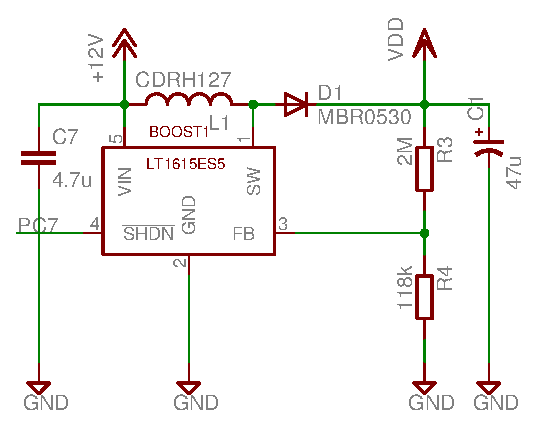
\includegraphics[scale=0.8]{implementation/figures/driver_interface_lcd_bias_circuit.eps}
 \caption{Boost converter circuit}
 \label{fig:lcd_boost_converter}
\end{figure}

\paragraph{Inductor Selection}

According to the datasheet, the value of the inductor $L_1$ can be determined by the following equation:

\begin{equation}
L_1=\frac{V_{out}-V_{in(min)}+V_{D}}{I_{limit}}\cdot t_{off}\label{IndSel}
\end{equation}

Where $V_D$ is the diode D1's forward voltage drop, $V_{out}$ the desired output voltage of the converter, $V_{in(min)}$ the minimum expected suppy voltage, and $I_{limit}$ the switching current limit of the converter device, between \unit{300}{\milli\ampere} and \unit{400}{\milli\ampere}, and $t_{off}$ the switching off-time of the converter device, typically \unit{400}{\nano\second}.

Using (\ref{IndSel}) with $V_{D}=\unit{0.4}{\volt}$, $I_{limit}=\unit{350}{\milli\ampere}$, $t_{off}=\unit{400}{\nano\second}$, $V_{out}=+\unit{22}{\volt}$, and $V_{in(min)}=\unit{11.5}{\volt}$ gives $L\approx\unit{12.45}{\micro\henry}$. The datasheet however suggests a value slightly smaller than calculated should be suitable with only slight decrease in maximum output current. Since the LCD requires very little current (estimated less than \unit{1}{\milli\ampere}, we used an inductor value of $\unit{10}{\micro\henry}$.


\paragraph{Output Voltage}

To obtain a $V_{bias}$ of $+\unit{22}{\volt}$, two resistors in the bias circuit provide a voltage divided feedback path from the output to the FB pin on the LT1615. The eqation relating the output voltage with the resistor values is

\begin{equation}
R_{3}=R_{4}\cdot\left(\frac{V_{bias}}{1.23}-1\right)
\end{equation}

 $R_{3}$ was chosen to be $\unit{2}{\mega\ohm}$ to limit current flowing from the output to ground, and a suitable $R_{4}$ of $\unit{118}{\kilo\ohm}$ was found.


\subsubsection{LCD Module Data Interface\label{sec:lcd_module_data_interface}}

The LCD's 8-bit interface was suitable to be connected to the AT90CAN128's external memory interface. This way the LCD becomes a memory-mapped periferal to the microcontroller, and all the control signals (Read and Write strobes, etc.), are handled by the memory controller.

The AT90CAN128's external memory interface uses Port A pins 0-7 as a multiplexed data and address bus which must be demultiplexed in order to offer seperate address and data busses. In operation, the external memory interface first puts out the address on the combined bus, followed by the data. The ALE (Address Latch Enable) signal signifies the difference \cite{AT90CAN}.

In order to provide seperate address and data busses for the LCD controller, a fast octal D-Type latch from NXP was chosen to latch the address from the AT90CAN128. The width of the ALE pulse, $t_{LHLL}$, provided by the AT90, is specified in the datasheet as

\nomenclature{$t_{LHLL}$}{The Address Latch Enable pulse width on the AT90CAN128's external memory interface}

\begin{equation}
t_{LHLL}=t_{CLCL}-15\, \nano\second
\end{equation}

where $t_{CLCL}$ is the main clock period. With the main clock running at $\unit{16}{\mega\hertz}$, $t_{LHLL}=\unit{48}{\nano\second}$.

\nomenclature{$t_{CLCL}$}{The main system clock period on the AT90CAN128.}

The 74LVC373A latch from NXP requires a minimum LE pulse width of $\unit{4.5}{\nano\second}$, so is suitable as a demultiplexing interface.

The external memory on the AT90CAN128 starts at address 0x1100h, and there are two possible registers to read/write to on the LCD controller. The LCD controller therefore has it's single address select pin connected to the LSB of the address lines output from the latch. Since only two addresses are required, the upper 8 address lines of the external memory interface were not used.

A logical combination of the lower byte address lines should be connected to the CS (Chip Select) line on the LCD controller. Since the external memory controller only outputs control signals when the requested memory operation is in external space, it is safe to ignore the upper byte address lines.

\nomenclature{CS}{Chip Select}

It was chosen to tie the 2nd bit of the address lines to CS. The resulting operations when interacting with the LCD controller are summarized in Table \ref{tab:lcd_memory_map}.

\begin{table}
\caption{Memory-mapped LCD Interface}
\label{tab:lcd_memory_map}
\centering{}
\begin{tabular}{|l|l|l|}
\hline 
Address  & Read Function  & Write Function\tabularnewline
\hline
\hline 
0x1101  & Status flag read  & Display data and parameter write\tabularnewline
\hline 
0x1102  & Display dada and cursor address read  & Command write\tabularnewline
\hline
\end{tabular}
\end{table}

\subsection{Software}

The system software running on the Telemetry module acts as a source of commands to the other modules on the network, and serves to meet the design outlined in Sec.\ \ref{sec:Driver-Interface-Module}. The majority of the software implemented is in support of the LCD hardware. The software supporting the buttons, knobs, and paddles is in comparison very simple.

\subsubsection{LCD Module Library}

An LCD module library was written to implement the entire command set of the SED1335. The functionality covers initializing the LCD Controller and screen from reset as well as setting up different layers and cursors, and drawing strings and bitmaps. Additionally, more complex drawing operations were implemented specifically to meet the requirements of the Driver Interface module, such as progress bars, underlines, a clock at the top of the screen, and the signal strength indicator. The parameter menu system was also implemented that allows the driver to scroll through the list of vehicle parameters to tune.

\subsubsection{Font Loading\label{sec:lcd_module_font_loading}}

The built-in font in the SED1335 LCD controller is only 5x7 pixels, and difficult to read. To display more readable text on the LCD screen, a custom 16x16 pixel fixed-width font for the character generator was developed in a series of steps:
\begin{enumerate}
 \item a 43 character subset of standard ASCII was chosen to be implemented, the capital letters A-Z, the numbers, and a few punctuation characters;
 \item next, a 688x16 pixel image was created in The Gimp image manipulation program. 16 pixel wide blocks were sectioned off, and using The Gimp's text tool, fixed width characters were drawn on the image at 16 pixel intervals;
  \item then, using The Gimp's python scripting interface, a small python script was written to pull the bitmap data out of the image and format it in such a way as could be placed in a standard c include file as a \emph{const char} array.
\end{enumerate}

A library was written for the Driver Interface module that at runtime loads this constant font data into the appropriate character generator ram on the LCD. Now, ASCII characters written to the character buffer in the LCD memory are drawn by the character generator and show up on the screen in the custom font. An image of the font used is shown in Fig.\ \ref{fig:driver_interface_font}.

\begin{figure}[htp]
 \centering
 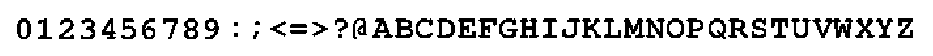
\includegraphics[scale=1]{implementation/figures/driver_interface_font.eps}
 \caption{Custom 16x16 pixel fixed-width font.}
 \label{fig:driver_interface_font}
\end{figure}

\subsubsection{I/O Library}

A small I/O Library was written to set up and manage the interrupts generated by the buttons, knobs, and paddles on the steering wheel.
 
%\subsubsection{Vehicle Diagnostics Library}
% 
% 
%\subsubsection{Vehicle Parameter Library}
% 
% 
% \subsubsection{Vehicle Dynamic Mode}


\subsubsection{CAN Interface}

A CAN Interface library was written to interface the rest of the Driver Interface module system software with events happening on the network. In particular, the CAN Interface library sends out upshift and downshift requests to the Transmission module when the I/O library indicates that a paddle has been pulled. The start and neutral find buttons operate in the same fashion. The Driver Interface module receives incoming dashboard data from the other modules, such as vehicle wheel speed, and Telemetry signal strength.

\subsubsection{Main Control Loop}
\section{CAN Diagnostic Tool}
\label{sec:implementation_candt}

\subsection{Overview}

\subsection{Scheduling}

\subsection{Injecting}

\subsection{Snooping}
